\section{Metodologia}
\label{sec:ctx-emb-metodologia}

O método proposto transforma a recuperação densa convencional em um processo de dois estágios no qual o mesmo modelo é empregado para indexar o \textit{corpus}, executar a busca inicial e produzir uma nova representação da consulta condicionada aos documentos recuperados. Seja $\mathcal{D}=\{d_1,\ldots,d_N\}$ o \textit{corpus}, $q$ uma consulta e $f_{\theta}(\cdot)$ o modelo de \textit{embeddings} parametrizado por $\theta$. Na primeira etapa, os documentos são codificados uma única vez,
\begin{equation}
    \mathbf{z}_{d}=f_{\theta}(d), \qquad d\in\mathcal{D},
\end{equation}
e a consulta é representada sem contexto:
\begin{equation}
    \mathbf{z}^{(0)}_{q}=f_{\theta}(I \oplus q),
\end{equation}
em que $I$ é a instrução da tarefa e $\oplus$ denota a concatenação textual. A similaridade cosseno entre $\mathbf{z}^{(0)}_{q}$ e os vetores do \textit{corpus} determina a lista inicial $\mathcal{C}_{10}(q)$, composta pelos dez documentos mais bem classificados.

Na segunda etapa, a consulta é reconstruída pela concatenação da instrução, da pergunta original e do prefixo $\mathcal{C}_{k}(q)\subseteq\mathcal{C}_{10}(q)$, contendo os $k$ primeiros documentos da lista inicial. O modelo gera então o vetor contextualizado
\begin{equation}
    \mathbf{z}^{(c)}_{q}
    =
    f_{\theta}\left(I\oplus q\oplus\mathcal{C}_{k}(q)\right).
\end{equation}
Esse vetor é comparado novamente com os mesmos vetores documentais previamente indexados. Portanto, a contextualização não exige uma segunda indexação do \textit{corpus}; somente as consultas são recodificadas. Diferentemente do RFG, não há geração autorregressiva de uma expansão textual intermediária. A ``expansão'' ocorre implicitamente no espaço vetorial, por meio da atenção do modelo sobre a consulta e o contexto recuperado.

\subsection{Conjuntos de dados}
\label{subsec:ctx-emb-dados}

Os experimentos foram realizados nos quatro conjuntos de recuperação descritos no Capítulo~3: BioASQ-RAG-Resplit, NarrativeQA-RAG, QASPER-RAG e Telco-DPR-RAG. Eles abrangem, respectivamente, os domínios biomédico, narrativo, científico e de telecomunicações.

\subsection{Ajuste fino dos modelos de \textit{embeddings} cientes de contexto}
\label{subsec:ctx-emb-ajuste}

O modelo-base adotado foi o \texttt{Qwen3-Embedding-4B}. Um adaptador LoRA independente foi treinado para cada conjunto de dados. A divisão de treino foi utilizada para otimização, a divisão de validação para selecionar o melhor \textit{checkpoint} e a divisão de teste exclusivamente para a avaliação final.

\subsubsection{Configuração de treinamento e seleção do modelo}
\label{subsubsec:ctx-emb-configuracao}

A Tabela~\ref{tab:config-ft-ctx-embedding} resume as configurações compartilhadas por todos os treinamentos principais. Os adaptadores foram aplicados às projeções de consulta e valor da atenção. Dessa forma, o codificador-base permaneceu congelado e somente 5.898.240 parâmetros foram atualizados, equivalentes a aproximadamente $0{,}1464\%$ do modelo com o adaptador.

\begin{table}[htbp]
\caption{Configurações gerais do ajuste fino do modelo de \textit{embeddings} ciente de contexto.}
\label{tab:config-ft-ctx-embedding}
\centering
\footnotesize
\begin{tabular}{ll}
\hline
\textbf{Configuração} & \textbf{Valor} \\ \hline
Modelo-base & \texttt{Qwen/Qwen3-Embedding-4B} \\
Parâmetros do modelo-base & 4.021.774.336 \\
Parâmetros LoRA treináveis & 5.898.240 (aprox.\ $0{,}1464\%$) \\
Projeções de atenção adaptadas & \texttt{q\_proj}, \texttt{v\_proj} \\
Posto LoRA ($r$) & 16 \\
Fator LoRA ($\alpha$) & 32 \\
\textit{Dropout} LoRA & 0,05 \\
Comprimento máximo da âncora & 3.072 \textit{tokens} \\
Limite da consulta & 512 \textit{tokens} \\
Limite por documento de contexto & 512 \textit{tokens} \\
Limite da passagem positiva & 512 \textit{tokens} \\
Número de documentos de contexto & 0--5 \\
Proporção com relevância garantida & 70\% dos exemplos com contexto \\
Taxa de aprendizado & $2\times10^{-5}$ \\
\textit{Warmup ratio} & 0,10 \\
Precisão numérica & \texttt{bfloat16} \\
Perda & \texttt{CachedMultipleNegativesRankingLoss} \\
Minilote interno da perda com \textit{cache} & 8 \\
Amostrador de lotes & Sem exemplos duplicados \\
Limite de \textit{checkpoints} & 3 \\ \hline
\end{tabular}
\end{table}

A Tabela~\ref{tab:config-ft-ctx-embedding-datasets} apresenta somente as configurações que variaram entre os conjuntos de dados. O lote indicado corresponde ao número de exemplos por dispositivo.

\begin{table}[htbp]
\caption{Configurações específicas do ajuste fino do modelo de \textit{embeddings} por conjunto de dados.}
\label{tab:config-ft-ctx-embedding-datasets}
\centering
\footnotesize
\begin{tabular}{lrrrr}
\hline
\textbf{Conjunto} &
\textbf{Lote} &
\textbf{Épocas} &
\textbf{Avaliação (passos)} &
\textbf{Salvamento (passos)} \\ \hline
BioASQ-RAG-Resplit & 32 & 10 & 50 & 50 \\
NarrativeQA-RAG & 32 & 10 & 50 & 50 \\
QASPER-RAG & 32 & 10 & 10 & 10 \\
Telco-DPR-RAG & 32 & 20 & 5 & 5 \\ \hline
\end{tabular}
\end{table}

Para acompanhar o treinamento e selecionar o melhor \textit{checkpoint}, utilizou-se o avaliador de recuperação de informação disponibilizado pela biblioteca \textit{Sentence Transformers}, denominado \texttt{InformationRetrievalEvaluator}. Esse componente recebe as consultas, o \textit{corpus} e os julgamentos de relevância da divisão de validação. A cada intervalo de avaliação indicado na Tabela~\ref{tab:config-ft-ctx-embedding-datasets}, o avaliador gera os \textit{embeddings} com o estado corrente do modelo, ordena os documentos pela similaridade cosseno e calcula as métricas de recuperação. Ao final do treinamento, seleciona-se o \textit{checkpoint} que obteve o maior nDCG@10 na validação. Assim, a escolha do modelo é determinada diretamente pela sua capacidade de recuperar e ordenar documentos relevantes, em vez de depender apenas do valor da perda contrastiva. Os treinamentos principais utilizaram dois aceleradores H100.

Além das configurações principais, foi treinada uma variante de contexto longo para o BioASQ-RAG-Resplit. Essa variante utilizou lote 128, dez épocas, avaliação e salvamento a cada 50 passos, limite de 2.048 \textit{tokens} por documento e passagem positiva e janela de 14.336 \textit{tokens}. O treinamento foi executado em quatro aceleradores H100.

Cada exemplo de treinamento é um par $(a_i,d_i^{+})$, no qual $a_i$ é uma âncora formada pela consulta, opcionalmente acrescida de contexto, e $d_i^{+}$ é um documento relevante segundo os julgamentos de relevância do conjunto de dados. Para consultas associadas a mais de um documento relevante, é criado um par para cada documento positivo. A âncora segue o formato:

\begin{verbatim}
Instruct: Given a web search query, retrieve relevant passages
that answer the query
Query:<consulta>
## Context:
doc 1:
<documento recuperado 1>
...
doc k:
<documento recuperado k>
\end{verbatim}

Para que um único adaptador opere nos dois estágios, o número de documentos de contexto é amostrado uniformemente entre zero e cinco para cada consulta. Consequentemente, parte dos exemplos contém apenas instrução e consulta, preservando a capacidade necessária à indexação e à busca inicial. Quando o exemplo possui contexto, são utilizados documentos previamente recuperados e ordenados pelo sistema de primeira etapa. Em $70\%$ desses casos, garante-se a presença de ao menos um documento relevante: caso nenhum dos documentos selecionados seja relevante, um deles é substituído, em posição aleatória, por um documento positivo. Nos demais casos, o contexto é mantido como recuperado, incluindo documentos potencialmente não relevantes. Essa mistura expõe o modelo tanto a evidências úteis quanto ao ruído que ocorre durante a inferência.

\begin{figure}[htbp]
    \centering
    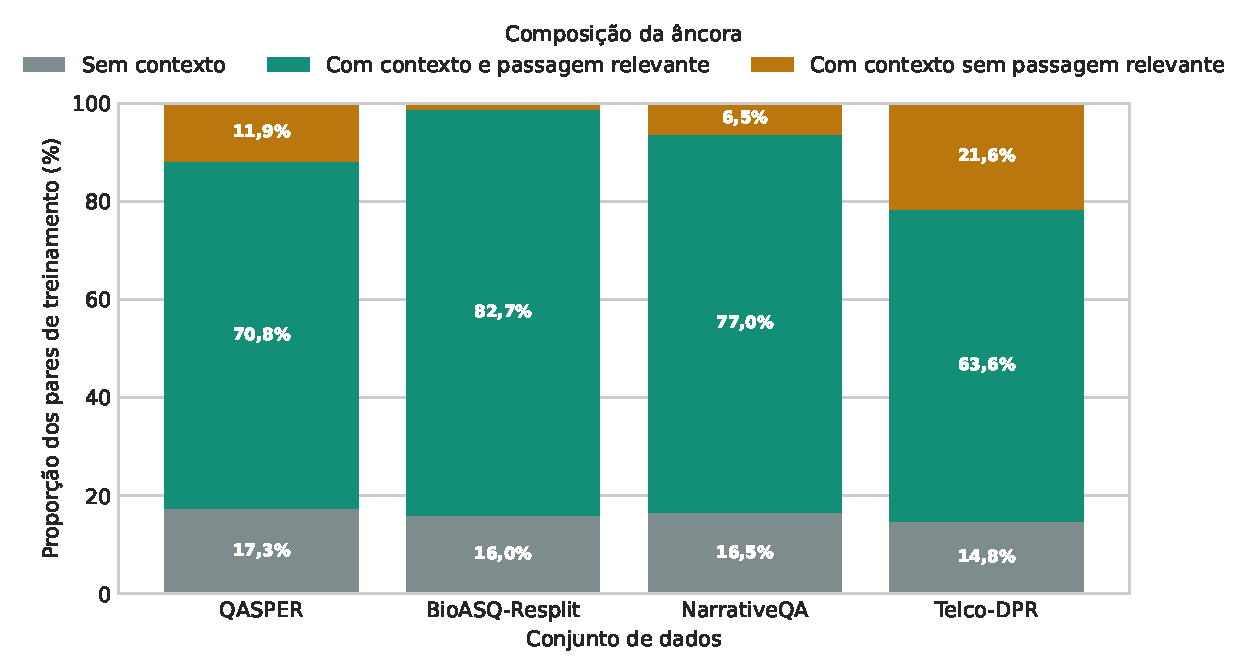
\includegraphics[width=0.75\textwidth]{reports/embedding_context_distribution/embedding_context_distribution_train.pdf}
    \caption{Distribuição dos pares de ajuste fino de \textit{embeddings} sem contexto, com contexto contendo ao menos uma passagem relevante e com contexto sem passagem relevante.}
    \label{fig:ctx-emb-distribuicao-contexto}
\end{figure}

A Figura~\ref{fig:ctx-emb-distribuicao-contexto} mostra a distribuição efetiva dos pares processados pela perda contrastiva. A fração sem contexto permaneceu próxima ao valor esperado de $1/6$: $17{,}30\%$ no QASPER, $15{,}95\%$ no BioASQ, $16{,}53\%$ no NarrativeQA e $14{,}77\%$ no Telco-DPR. A proporção de pares com contexto e ao menos uma passagem relevante foi de $70{,}77\%$, $82{,}69\%$, $77{,}01\%$ e $63{,}59\%$, respectivamente. Já os contextos sem passagem relevante representaram $11{,}93\%$, $1{,}36\%$, $6{,}47\%$ e $21{,}64\%$. A presença dessa última categoria é deliberada: ela aproxima o treinamento da inferência, na qual a primeira recuperação não garante evidência relevante. A baixa proporção observada no BioASQ decorre tanto do maior número de passagens relevantes por consulta quanto da expansão de uma mesma âncora em múltiplos pares positivos.

Para consultas associadas a múltiplas passagens relevantes, a mesma âncora origina um par para cada positivo. Por isso, a quantidade de pares contrastivos da Tabela~\ref{tab:ctx-emb-pares} pode superar a quantidade de consultas.

\begin{table}[htbp]
\caption{Quantidade de pares utilizados no ajuste fino contextual, discriminada por divisão e presença de contexto.}
\label{tab:ctx-emb-pares}
\centering
\small
\begin{tabular}{lrrrr}
\hline
& \multicolumn{2}{c}{\textbf{Treino}}
& \multicolumn{2}{c}{\textbf{Validação}} \\
\cline{2-5}
\textbf{Conjunto} &
\textbf{Total} &
\textbf{Sem contexto} &
\textbf{Total} &
\textbf{Sem contexto} \\ \hline
BioASQ-RAG-Resplit & 29.385 & 4.687 & 7.333 & 1.602 \\
NarrativeQA-RAG    & 32.747 & 5.412 & 3.461 & 556 \\
QASPER-RAG         & 3.815  & 660   & 1.913 & 297 \\
Telco-DPR-RAG      & 975    & 144   & 243   & 47 \\ \hline
\end{tabular}
\end{table}

As consultas foram limitadas a 512 \textit{tokens}; cada documento de contexto e cada passagem positiva também foi limitado a 512 \textit{tokens}. O comprimento máximo da âncora foi fixado em 3.072 \textit{tokens}. Quando a concatenação ultrapassava esse limite, documentos eram removidos a partir do final da lista até que a sequência coubesse na janela definida. Essa política preserva prioritariamente a consulta e os documentos mais bem classificados.

O objetivo de treinamento foi a \texttt{CachedMultipleNegativesRankingLoss}. Para um lote com $B$ pares, os demais documentos positivos do lote atuam como negativos para a âncora $a_i$; não foram adicionados negativos difíceis explícitos. Em termos simplificados, minimiza-se
\begin{equation}
    \mathcal{L}
    =
    -\frac{1}{B}
    \sum_{i=1}^{B}
    \log
    \frac{
        \exp\left(s(f_{\theta}(a_i),f_{\theta}(d_i^{+}))/\tau\right)
    }{
        \sum_{j=1}^{B}
        \exp\left(s(f_{\theta}(a_i),f_{\theta}(d_j^{+}))/\tau\right)
    },
\end{equation}
em que $s(\cdot,\cdot)$ é a similaridade cosseno e $\tau$ é a temperatura empregada pela função de perda. A versão com \textit{cache} permite utilizar um lote contrastivo maior do que o lote efetivamente codificado em cada passo, reduzindo o consumo de memória. Adicionalmente, o amostrador evita exemplos duplicados dentro do mesmo lote, prevenindo falsos negativos triviais.

\subsection{Recuperação contextual em dois estágios}
\label{subsec:ctx-emb-dois-estagios}

Antes de receber consultas, o \textit{corpus} é indexado uma única vez. Cada documento é codificado sem contexto, e seu vetor normalizado é armazenado no índice. Essa operação corresponde à preparação \textit{offline} do sistema e é compartilhada pelos dois estágios de recuperação.

No primeiro estágio, a consulta é formada apenas pela instrução e pela pergunta. O mesmo adaptador contextual gera $\mathbf{z}^{(0)}_q$, que é comparado com o índice para recuperar os dez documentos mais similares. Essa etapa não dispõe de contexto externo e, por isso, depende dos exemplos sem contexto incluídos durante o ajuste fino.

No segundo estágio, os primeiros $k$ documentos da lista inicial são concatenados à consulta, com $k\in\{1,3,5,7,10\}$. Cada documento é truncado individualmente em 512 \textit{tokens}, mas não se aplica o limite de 3.072 \textit{tokens} usado durante o treinamento: nenhum documento é removido em razão do comprimento total da entrada. Como o maior caso contém dez documentos, a entrada permanece dentro da janela suportada pelo modelo. O vetor contextualizado $\mathbf{z}^{(c)}_q$ é então comparado novamente com todo o \textit{corpus}, e não apenas com os dez candidatos iniciais. Assim, a segunda busca pode recuperar documentos ausentes da primeira lista.

Essa arquitetura possui três propriedades. Primeiro, o índice documental é compartilhado entre os dois estágios. Segundo, os documentos que formam o contexto são obtidos exclusivamente pela busca inicial, sem uso dos julgamentos de relevância no teste. Terceiro, o modelo contextual é robustecido durante o treinamento com quantidades variáveis de contexto e com exemplos sem contexto. A etapa de injeção controlada de documentos relevantes é restrita à construção dos dados de treinamento e validação.

\section{Procedimentos Experimentais}
\label{sec:ctx-emb-procedimentos}

Todas as avaliações foram executadas com lote de codificação 128 e \textit{backend} \texttt{vLLM}, utilizando a divisão de teste e o protocolo MTEB. Os experimentos reportam nDCG@10, MAP@10 e Recall@10; a escolha de $k$ é apresentada como análise ablatória descritiva sobre esses resultados.

\subsection{Experimento 1: influência da quantidade de contexto}

O primeiro experimento avaliou o modelo contextual com $k\in\{1,3,5,7,10\}$, com o objetivo de determinar como a quantidade de documentos fornecida ao segundo estágio afeta a recuperação e identificar um valor de $k$ adequado de forma geral. Em todas as condições, o primeiro estágio recuperou dez documentos. Cada documento fornecido ao segundo estágio foi limitado a 512 \textit{tokens}, sem remoção de documentos em função do comprimento total da entrada.

Para QASPER-RAG, a primeira recuperação foi restrita aos segmentos pertencentes ao artigo associado à pergunta, em conformidade com o protocolo do conjunto; nos demais casos, a busca foi realizada sobre o \textit{corpus} completo. O segundo estágio pesquisou novamente o mesmo espaço documental completo. A métrica principal foi nDCG@10, e MAP@10 e Recall@10 foram utilizadas como medidas complementares. O melhor $k$ geral foi definido pela média macro de nDCG@10 nos quatro conjuntos.

\subsection{Experimento 2: comparação com as abordagens de referência}

O segundo experimento comparou cinco condições:
\begin{enumerate}
    \item \textbf{Modelo-base}: \texttt{Qwen3-Embedding-4B} sem ajuste fino e sem contexto;
    \item \textbf{FT sem contexto}: modelo de \textit{embeddings} ajustado apenas com pares consulta--documento, apresentado no Capítulo~4;
    \item \textbf{RFG}: expansão fundamentada em recuperação do Capítulo~5, utilizando a configuração geral $k=7$, concatenação da consulta com a expansão, \textit{embedding} base e gerador base;
    \item \textbf{FT contextual sem contexto}: adaptador proposto operando apenas no primeiro estágio, com instrução e consulta;
    \item \textbf{FT contextual com contexto}: adaptador proposto no segundo estágio, utilizando o melhor valor geral de $k$ identificado no Experimento~1.
\end{enumerate}

Essa comparação permite separar o ganho do ajuste fino convencional, o efeito de treinar o adaptador contextual sem fornecer contexto na inferência e o ganho adicional obtido pela segunda recuperação. A condição RFG também permite contrastar a contextualização direta no espaço vetorial com a geração de uma expansão textual.

\subsection{Experimento 3: influência do comprimento dos documentos}

O terceiro experimento investigou se o limite de 512 \textit{tokens} por documento restringia o desempenho no BioASQ-RAG-Resplit. Foram avaliadas três condições. Na primeira, o adaptador principal foi treinado e avaliado com documentos de até 512 \textit{tokens}. Na segunda, o mesmo adaptador foi mantido, mas os cinco documentos do segundo estágio puderam conter até 2.048 \textit{tokens}. Na terceira, treinou-se uma variante específica do BioASQ com documentos e passagens positivas de até 2.048 \textit{tokens}, janela de 14.336 \textit{tokens} e lote 128; essa variante foi avaliada com $k\in\{1,3,5\}$.

O contraste entre as duas primeiras condições isola o efeito de aumentar o contexto somente na inferência. A terceira condição verifica se a exposição a sequências longas durante o treinamento torna o modelo mais capaz de aproveitar esse conteúdo adicional. Como a variante longa também utiliza um lote maior, seus resultados são interpretados como uma ablação conjunta, e não como uma estimativa causal exclusiva do comprimento.

\section{Resultados}
\label{sec:ctx-emb-resultados}

\subsection{Influência da quantidade de contexto}

A Tabela~\ref{tab:ctx-emb-k} apresenta o nDCG@10 obtido ao variar a quantidade de documentos no segundo estágio. O melhor resultado macro foi alcançado com $k=5$, com 0,7514, seguido de perto por $k=3$, com 0,7511. O uso de dez documentos reduziu a média para 0,7299, mostrando que a adição irrestrita de evidências pode introduzir ruído.

\begin{table}[htbp]
\caption{Influência do número de documentos fornecidos ao segundo estágio. Os valores entre parênteses representam a variação absoluta do nDCG@10 em relação ao modelo-base sem ajuste fino. A última coluna apresenta a média macro entre os conjuntos.}
\label{tab:ctx-emb-k}
\centering
\scriptsize
\resizebox{\textwidth}{!}{
\begin{tabular}{lccccc}
\hline
\textbf{Configuração} &
\textbf{BioASQ-resplit} &
\textbf{NarrativeQA} &
\textbf{QASPER} &
\textbf{Telco-DPR} &
\textbf{Média} \\ \hline

Baseline &
\cellcolor{resultbaseline}0,78468 &
\cellcolor{resultbaseline}0,74365 &
\cellcolor{resultbaseline}0,56841 &
\cellcolor{resultbaseline}0,52933 &
\cellcolor{resultbaseline}0,65652 \\

$k=1$ &
\cellcolor{resultgain}\textbf{0,81840 (+0,03372)} &
\cellcolor{resultgain}0,81810 (+0,07445) &
\cellcolor{resultgain}0,57634 (+0,00793) &
\cellcolor{resultgain}0,70748 (+0,17815) &
\cellcolor{resultgain}0,73008 (+0,07356) \\

$k=3$ &
\cellcolor{resultgain}\textbf{0,81840 (+0,03372)} &
\cellcolor{resultgain}0,83416 (+0,09051) &
\cellcolor{resultgain}0,61992 (+0,05151) &
\cellcolor{resultgain}0,73179 (+0,20246) &
\cellcolor{resultgain}0,75107 (+0,09455) \\

$k=5$ &
\cellcolor{resultgain}0,81539 (+0,03071) &
\cellcolor{resultgain}\textbf{0,83806 (+0,09441)} &
\cellcolor{resultgain}\textbf{0,62032 (+0,05191)} &
\cellcolor{resultgain}0,73192 (+0,20259) &
\cellcolor{resultgain}\textbf{0,75142 (+0,09490)} \\

$k=7$ &
\cellcolor{resultgain}0,81261 (+0,02793) &
\cellcolor{resultgain}0,83746 (+0,09381) &
\cellcolor{resultgain}0,61163 (+0,04322) &
\cellcolor{resultgain}\textbf{0,73884 (+0,20951)} &
\cellcolor{resultgain}0,75013 (+0,09362) \\

$k=10$ &
\cellcolor{resultgain}0,80541 (+0,02073) &
\cellcolor{resultgain}0,79417 (+0,05052) &
\cellcolor{resultgain}0,59346 (+0,02505) &
\cellcolor{resultgain}0,72665 (+0,19732) &
\cellcolor{resultgain}0,72992 (+0,07341) \\ \hline

\end{tabular}
}
\end{table}

A escolha ótima variou entre os conjuntos. BioASQ obteve o mesmo nDCG@10 com $k=1$ e $k=3$; NarrativeQA e QASPER apresentaram seus melhores resultados contextuais com $k=5$; Telco-DPR atingiu o máximo com $k=7$. A degradação do NarrativeQA de 0,8381 em $k=5$ para 0,7942 em $k=10$ foi a principal responsável pela queda da média nessa configuração.

A Tabela~\ref{tab:ctx-emb-metricas-k5} detalha as três métricas para $k=5$. A média macro foi 0,7514 em nDCG@10, 0,6695 em MAP@10 e 0,8236 em Recall@10.

\begin{table}[htbp]
    \centering
    \caption{Resultados do segundo estágio com $k=5$.}
    \label{tab:ctx-emb-metricas-k5}
    \begin{tabular}{lrrr}
        \toprule
        Conjunto & nDCG@10 & MAP@10 & Recall@10 \\
        \midrule
        BioASQ-RAG-Resplit & 0,8154 & 0,6542 & 0,7438 \\
        NarrativeQA-RAG   & 0,8381 & 0,8181 & 0,8993 \\
        QASPER-RAG        & 0,6203 & 0,5215 & 0,7719 \\
        Telco-DPR-RAG     & 0,7319 & 0,6841 & 0,8795 \\
        \midrule
        Média macro       & 0,7514 & 0,6695 & 0,8236 \\
        \bottomrule
    \end{tabular}
\end{table}

\subsection{Comparação com as abordagens de referência}

A Tabela~\ref{tab:ctx-emb-comparacao} compara o melhor valor geral, $k=5$, com as abordagens de referência. O ajuste fino sem contexto elevou a média de 0,6565 para 0,7434. O adaptador contextual sem documentos na entrada obteve 0,7436, diferença de apenas 0,0002, mostrando que o treinamento misto preservou a capacidade do primeiro estágio. A inclusão dos cinco documentos aumentou a média para 0,7514.

\begin{table}[htbp]
    \centering
    \caption{Comparação de nDCG@10 com as abordagens de referência.}
    \label{tab:ctx-emb-comparacao}
    \begin{tabular}{lrrrrr}
        \toprule
        Método & BioASQ & NarrativeQA & QASPER & Telco-DPR & Média macro \\
        \midrule
        Modelo-base & 0,7847 & 0,7437 & 0,5684 & 0,5293 & 0,6565 \\
        FT sem contexto & \textbf{0,8264} & 0,8235 & \textbf{0,6371} & 0,6867 & 0,7434 \\
        RFG ($k=7$, concat.) & 0,7880 & 0,7935 & 0,6209 & 0,5530 & 0,6889 \\
        FT contextual sem contexto & 0,8159 & 0,8225 & 0,6252 & 0,7109 & 0,7436 \\
        FT contextual, $k=5$ & 0,8154 & \textbf{0,8381} & 0,6203 & \textbf{0,7319} & \textbf{0,7514} \\
        \bottomrule
    \end{tabular}
\end{table}

Em média, o segundo estágio contextual superou o modelo-base em 0,0949, o ajuste fino sem contexto em 0,0080, o próprio adaptador sem contexto em 0,0078 e a configuração RFG comparada em 0,0626. O ganho sobre o primeiro estágio concentrou-se no NarrativeQA ($+0,0156$) e no Telco-DPR ($+0,0210$). BioASQ permaneceu praticamente estável ($-0,0005$), e QASPER apresentou redução de 0,0048.

\subsection{Influência do comprimento dos documentos}

A Tabela~\ref{tab:ctx-emb-contexto-longo} apresenta a ablação realizada no BioASQ. Aumentar o limite para 2.048 \textit{tokens} apenas na inferência, mantendo o adaptador treinado com 512 \textit{tokens}, produziu 0,8149 em $k=5$, valor ligeiramente inferior aos 0,8154 do protocolo principal. Quando o modelo também foi treinado com contexto longo e lote 128, o melhor resultado foi 0,8226 em $k=3$.

\begin{table}[htbp]
    \centering
    \caption{nDCG@10 no BioASQ ao variar o comprimento dos documentos de contexto.}
    \label{tab:ctx-emb-contexto-longo}
    \begin{tabular}{lrrr}
        \toprule
        Treinamento / inferência & $k=1$ & $k=3$ & $k=5$ \\
        \midrule
        512 / 512 \textit{tokens} & 0,8184 & 0,8184 & 0,8154 \\
        512 / 2.048 \textit{tokens} & -- & -- & 0,8149 \\
        2.048 / 2.048 \textit{tokens}, lote 128 & 0,8207 & \textbf{0,8226} & 0,8169 \\
        \bottomrule
    \end{tabular}
\end{table}

Em $k=3$, a variante longa superou o modelo principal em 0,0042; em $k=5$, a diferença foi 0,0015. Portanto, o treinamento compatível com sequências maiores produziu uma melhora pequena, enquanto aumentar somente a janela de inferência não trouxe benefício.

\section{Discussão}
\label{sec:ctx-emb-discussao}

Os resultados sustentam, em primeiro lugar, que um único adaptador pode atender às duas etapas. A diferença de apenas 0,0002 na média de nDCG@10 entre o ajuste fino sem contexto e o adaptador contextual no primeiro estágio indica que a mistura de exemplos preservou a capacidade de codificar consultas sem documentos de apoio. Essa propriedade é indispensável, pois a primeira recuperação ocorre antes de qualquer contexto estar disponível.

Em segundo lugar, os documentos recuperados podem orientar diretamente a representação vetorial da consulta. O ganho macro de 0,0078 sobre o mesmo adaptador sem contexto é modesto, mas aparece sem gerar uma expansão textual intermediária. NarrativeQA e Telco-DPR foram os conjuntos mais beneficiados, sugerindo que evidências narrativas ou terminologia técnica recuperada podem complementar a formulação original da pergunta.

O efeito depende, contudo, da quantidade e da qualidade do contexto. O melhor compromisso geral foi $k=5$, mas nenhum valor foi ótimo para todos os conjuntos. Quando todos os dez documentos foram preservados na entrada, NarrativeQA sofreu queda acentuada. Esse resultado mostra que a ampla janela do modelo não elimina a deriva semântica: documentos adicionais podem competir pela atenção e deslocar o vetor para informações secundárias. O fato de o treinamento principal apresentar no máximo cinco documentos também cria uma mudança de distribuição nas avaliações com $k=7$ e $k=10$.

No QASPER, o adaptador sem contexto ainda superou todas as configurações do segundo estágio. Como as perguntas são vinculadas a artigos específicos, segmentos sobre aspectos secundários do mesmo trabalho podem parecer semanticamente próximos sem fornecer a evidência necessária. No BioASQ, a estabilidade sugere que a terminologia da própria consulta já oferece um sinal discriminativo forte, limitando o benefício marginal do contexto.

A variante de contexto longo do BioASQ alcançou sua melhor melhora em $k=3$, mas a diferença de 0,0042 é pequena. Além disso, o experimento alterou simultaneamente o comprimento das sequências e o lote de treinamento, de 32 para 128. Portanto, o resultado não permite atribuir causalmente o ganho apenas aos 2.048 \textit{tokens}. A ausência de melhora ao ampliar somente a inferência reforça que mais texto não é automaticamente mais informação útil.

Em relação ao RFG do Capítulo~5, o método proposto mantém a fundamentação em documentos recuperados, mas substitui a geração autorregressiva por uma única codificação contextual. A comparação favoreceu o modelo contextual, porém não isola apenas essa diferença: a configuração RFG utiliza modelos e um procedimento de expansão distintos. Além disso, este capítulo não mediu latência, memória ou consumo energético. A redução de custo permanece uma consequência arquitetural plausível, mas requer medição controlada ponta a ponta.

Finalmente, os resultados correspondem a uma execução por configuração, sem repetição com diferentes sementes ou testes de significância. Diferenças pequenas devem ser interpretadas descritivamente. A injeção de uma passagem relevante ocorre somente durante treino e validação; no teste, o segundo estágio depende integralmente da qualidade da recuperação inicial. As métricas também avaliam alinhamento para recuperação, e não ``alucinação'' vetorial de forma direta.

\section{Conclusões}
\label{sec:ctx-emb-conclusoes}

Este capítulo apresentou um modelo de \textit{embeddings} ciente de contexto para recuperação densa em dois estágios. O \texttt{Qwen3-Embedding-4B} foi ajustado com âncoras contendo entre zero e cinco documentos recuperados, combinando exemplos com evidência relevante, contexto ruidoso e ausência de contexto. Com isso, o mesmo adaptador pôde executar a busca inicial e, em seguida, recodificar a consulta com os documentos recuperados, sem alterar o índice do \textit{corpus} e sem recorrer a um LLM gerador.

Na média dos quatro conjuntos de teste, a melhor configuração contextual, com $k=5$, alcançou nDCG@10 de 0,7514, frente a 0,7436 no mesmo adaptador sem contexto, 0,7434 no ajuste fino convencional, 0,6889 no RFG comparado e 0,6565 no modelo-base. A melhora contextual concentrou-se no NarrativeQA e no Telco-DPR; BioASQ permaneceu estável e QASPER apresentou sensibilidade ao ruído. Preservar dez documentos na entrada reduziu a qualidade média, confirmando que a capacidade de processar sequências longas não substitui a seleção de evidência.

O treinamento com documentos de até 2.048 \textit{tokens} produziu uma melhora pequena no BioASQ, enquanto ampliar apenas a entrada de inferência não trouxe benefício. Como continuidade, recomenda-se investigar seleção adaptativa de $k$, filtragem ou reordenação das passagens, treinamento com mais de cinco documentos, diferentes níveis de ruído e destilação de expansões RFG. Uma avaliação completa deve ainda incluir latência ponta a ponta, vazão, memória, consumo energético e repetição com múltiplas sementes.
